\documentclass[]{article}
\usepackage{lmodern}
\usepackage{amssymb,amsmath}
\usepackage{ifxetex,ifluatex}
\usepackage{fixltx2e} % provides \textsubscript
\ifnum 0\ifxetex 1\fi\ifluatex 1\fi=0 % if pdftex
  \usepackage[T1]{fontenc}
  \usepackage[utf8]{inputenc}
\else % if luatex or xelatex
  \ifxetex
    \usepackage{mathspec}
  \else
    \usepackage{fontspec}
  \fi
  \defaultfontfeatures{Ligatures=TeX,Scale=MatchLowercase}
\fi
% use upquote if available, for straight quotes in verbatim environments
\IfFileExists{upquote.sty}{\usepackage{upquote}}{}
% use microtype if available
\IfFileExists{microtype.sty}{%
\usepackage{microtype}
\UseMicrotypeSet[protrusion]{basicmath} % disable protrusion for tt fonts
}{}
\usepackage[margin=1in]{geometry}
\usepackage{hyperref}
\hypersetup{unicode=true,
            pdftitle={Measuring Hospital Acquired Infection Rates under Incomplete Sampling},
            pdfauthor={Derek Sonderegger, Jason Sahl, and Paul Keim},
            pdfborder={0 0 0},
            breaklinks=true}
\urlstyle{same}  % don't use monospace font for urls
\usepackage{graphicx,grffile}
\makeatletter
\def\maxwidth{\ifdim\Gin@nat@width>\linewidth\linewidth\else\Gin@nat@width\fi}
\def\maxheight{\ifdim\Gin@nat@height>\textheight\textheight\else\Gin@nat@height\fi}
\makeatother
% Scale images if necessary, so that they will not overflow the page
% margins by default, and it is still possible to overwrite the defaults
% using explicit options in \includegraphics[width, height, ...]{}
\setkeys{Gin}{width=\maxwidth,height=\maxheight,keepaspectratio}
\IfFileExists{parskip.sty}{%
\usepackage{parskip}
}{% else
\setlength{\parindent}{0pt}
\setlength{\parskip}{6pt plus 2pt minus 1pt}
}
\setlength{\emergencystretch}{3em}  % prevent overfull lines
\providecommand{\tightlist}{%
  \setlength{\itemsep}{0pt}\setlength{\parskip}{0pt}}
\setcounter{secnumdepth}{0}
% Redefines (sub)paragraphs to behave more like sections
\ifx\paragraph\undefined\else
\let\oldparagraph\paragraph
\renewcommand{\paragraph}[1]{\oldparagraph{#1}\mbox{}}
\fi
\ifx\subparagraph\undefined\else
\let\oldsubparagraph\subparagraph
\renewcommand{\subparagraph}[1]{\oldsubparagraph{#1}\mbox{}}
\fi

%%% Use protect on footnotes to avoid problems with footnotes in titles
\let\rmarkdownfootnote\footnote%
\def\footnote{\protect\rmarkdownfootnote}

%%% Change title format to be more compact
\usepackage{titling}

% Create subtitle command for use in maketitle
\providecommand{\subtitle}[1]{
  \posttitle{
    \begin{center}\large#1\end{center}
    }
}

\setlength{\droptitle}{-2em}

  \title{Measuring Hospital Acquired Infection Rates under Incomplete Sampling}
    \pretitle{\vspace{\droptitle}\centering\huge}
  \posttitle{\par}
    \author{Derek Sonderegger, Jason Sahl, and Paul Keim}
    \preauthor{\centering\large\emph}
  \postauthor{\par}
      \predate{\centering\large\emph}
  \postdate{\par}
    \date{2019-05-20}


\begin{document}
\maketitle

\hypertarget{abstract}{%
\subsection{Abstract}\label{abstract}}

\emph{Clostridioides difficile} is a diarrheagenic pathogen often
associated with healthcare-acquired infections and is a common secondary
infection in patients on strong antibiotic therapy. Identifying if the
pathogen was already present in/on the patient versus first encountered
at the healthcare facility and due to a transmission between patients
has monetary implications in regard to U.S. Medicare reimbursements as
well as informing clinical sanitation procedures. By genotyping \emph{C.
diff} disease strains among all patients with the disease, we could
detect transmission events between patients therefore calculate the HAI
rate. Because genotyping strains from every \emph{C. diff} positive
patient would be prohibitively expensive, we consider various levels of
sampling effort and demonstrate that the sample HAI rate is an
underestimate of the population HAI rate and propose a bias-correction
procedure. We apply the the bias-corrected estimator to two clinical
populations where nearly the full population was genotyped as well as to
simulated population. The bias-corrected estimator appears to work well
but performance degrades as sampling and transmission percentages
decrease.

\hypertarget{introduction}{%
\subsection{Introduction}\label{introduction}}

\emph{Clostridioides difficile} is a ubiquitous, diarrheagenic,
bacterial pathogen often associated with healthcare-acquired infections
(HAIs) that can cause a range of symptoms from mild, self-limiting
disease to toxic megacolon and death. Treatment for symptomatic \emph{C.
diff} infections is an antibiotic course of metronidazole, vancomycin,
or fidaxomicin. Individuals carrying \emph{C. diff} in their dermis or
gastro-intestinal tract can remain asymptomatic due to competitive
pressures in the microbiome. Because \emph{C. diff} displays a wide
range of antibiotic resistance, when patients are treated with
antibiotics to address another infection, the competitive suppression of
\emph{C. diff} is removed and the patient endures a secondary infection.
Alternatively, the patient undergoing an antibiotic course at a
healthcare facility might first be exposed to \emph{C. diff} at the
facility.

The different sources of \emph{C. diff} has substantial implications to
the healthcare facility. In the United States, Medicare reimbursement
rates are informed by the facilities overall rate of HAIs with
incentives and penalties up to \(\pm 1 \%\) which could be millions
dollars (???) for a mid-sized regional hospital. If patients are
primarily encountering \emph{C. diff} within the facility, then
sanitation procedures within the hospital could affect the HAI rate
providers should be concerned about strains endemic to the healthcare
facility developing resistance to the treatment course. If patients are
bringing the pathogen, then options for reducing HAI rates are
substantially reduced.

Phylogenetic studies utilizing whole genome sequencing have investigated
the spread of fluoroquinolone-resistant strains of \emph{C. diff}
(CITATION). These same techniques can identify clustering of strains
within a healthcare facility versus those present in the environment
outside the facility. The methods in this paper require an initial
clustering step that classifies patients into clusters, where a cluster
contains at least one patient. If all \(N\) patients bring their own
strain into the facility, then we should observe \(N\) different
clusters, each with a cluster size of one. Conversely, if all the
infections are a result of a single \emph{C. diff} source, we would
observe a single cluster with a cluster size of \(N\).

Medicare defines a \emph{C. diff} case as being a HAI if the diagnosis
occurs more than three days after admittance. In this paper, we will
instead define case as healthcare-acquired if there is evidence that it
occurred via a patient-to-patient transmission. We define a healthcare
facility's \emph{C. diff} HAI rate as the ratio of patient-to-patient
transmissions to the total number of \(C. diff\) cases.

The problem of detecting patient-to-patient transmission could be
considered as a network graph problem with each patient denoted by a
vertex and a transmission as an edge. However, most network graph
analysis methods assume that the graph is fully known and informally
most network analysis experts recommend needing at least \(80\%\) of the
nodes/edges being observed. In our context, there are \(N\) nodes and
\(N \times N\) possible edges, but most of those edges are unobserved.

\hypertarget{materials-and-methods}{%
\subsection{Materials and Methods}\label{materials-and-methods}}

\hypertarget{data-sources-clinical}{%
\paragraph{Data Sources: Clinical}\label{data-sources-clinical}}

Eyre \emph{et al} (2013) {[}1{]} describes a study in Oxfordshire,
United Kingdom where they genotyped nearly all cases of
\emph{Clostridium difficile} infections in Oxfordshire. Using
single-nucleotide polymorphisms (SNPs), they created clusters of
infection lineages by grouping cases that differed by two or fewer SNPs
using complete linkage clustering. Most (536 / 811 = 66\%), of the
patients where in a cluster by themselves, i.e.~their \emph{C.difficile}
case was more than two SNPs different than all other cases. Another 28\%
of the patients were in cluster groups between 2-13 and 50 patients
(6\%) were in one large cluster.

Eyre \emph{et al} {[}1{]} justified their choice of \(\le 2\) SNPs
differences by looking at within patient differences, but the cluster
size distributions were not sensitive to small changes in this
threshold, but the extreme choice of a threshold of 10 SNPs differences
results in an additional large cluster of 29 patients.

Flagstaff Medical Center, a regional hospital in Northern Arizona,
attempted to collect samples from every \emph{C. diff} case that was
diagnosed from \textbf{20XX-20XX}. The samples were genotyped at PMI and
we again used the two SNP differences to define clusters.

\hypertarget{data-sources-simulated-populations}{%
\paragraph{Data Sources: Simulated
Populations}\label{data-sources-simulated-populations}}

Both the Oxfordshire and Flagstaff data could be reasonably modeled
using a mixture of two distributions to separate the small clusters
sizes from the large. We chose to model the small clusters sizes using a
truncated Poisson distribution with the zero truncated out. The large
cluster sizes were modeled from a discretized logNormal distribution.

\[n_i | \lambda \sim \textrm{TPoisson}(\lambda) \textrm{ with probability } \rho\]
\[n_i | \lambda \sim \textrm{logNormal}(\mu, \sigma) \textrm{ with probability } 1 - \rho\]

for \(i\) in \(\mathcal{I}\).

\hypertarget{estimators}{%
\paragraph{Estimators}\label{estimators}}

First we denote \(N\) as the total number of patients, and \(\alpha\) as
the proportion of patients that are sampled (therefore \(\alpha N\)
patients are randomly sampled). We define \(n_i\) be the true size of
the \(i\)th cluster, and \(m_i\) as the observed size of the \(i\)th
cluster. We denote the total number of clusters in the population as
\(||\mathcal{I}||\) where \(\mathcal{I}\) is the set of cluster indices.
Because \(||\mathcal{I}||\) can be thought of as the number of non-HAI
cases, defining the true HAI rate as \(\gamma\) we have

\[\gamma = \frac{N - ||\mathcal{I}||}{N} = 1 - \frac{||\mathcal{I}||}{N}\]

We first consider the simplest data generating model of latent cluster
sizes

\[n_i \stackrel{iid}{\sim} \textrm{TPoisson}(\lambda) \; \textrm{for} \; i\in \mathcal{I}\]

Regardless of how the cluster sizes \(n_i\) are generated, the simple
random sampling results

\[m_i | n_i \sim \textrm{ZTHyperGeometric}(n_i, \; N-n_i, \;\alpha N) \; \textrm{for}\; i \in I\]

where \(I\) is a subset of \(\mathcal{I}\) and the ZT represents the
zero truncated out. This distribution is subject to the requirement that
\(\sum m_i = \alpha N\), but because in the clinical examples, the
number of clusters is quite high, the correlation between any two
clusters is small and we chose to ignore this and assume independence
among the \(m_i | n_i\) observations.

Results for the zero truncated hypergeometric distribution rely of
knowing, or approximating, the hypergeometric distribution probability
of observing a zero

\[f(0|n_i) =  \frac{ {n_i \choose 0}{N-n_i \choose \alpha N} }{ {N \choose \alpha N}}\]

Notice that \(\alpha\) and \(f(0|n_i)\) are inversely related and we
could crudely approximate

\[f(0|n_i) \approx 1-\alpha\]

Furthermore

\[E[m_i] = E[ E(m_i|n_i)] = E[ (1-f(0|n_i))^{-1} \;\alpha \;n_i]\]

Utilizing this information, can derive two different estimators for
\(n_i\).

\begin{enumerate}
\def\labelenumi{\arabic{enumi}.}
\tightlist
\item
  The plug-in estimator that ignores the RHS expectation, and
  approximates \(\left[ 1-f(0)\right]^{-1} \approx \alpha^{-1}\). This
  results in \(\widehat{n}_i = m_i\).
\item
  Ignoring the expectations, we could utilize the actual hypergeometric
  function for \(f(0|n_i)\) and solve the following equation for
  \(\widehat{n}_i\). This solution needs to be solved via numerical
  methods because the ``chooses'' in \(f(0|\widehat{n}_i)\).
\end{enumerate}

\[m_i =  (1-f(0|\widehat{n}_i))^{-1} \;\alpha \; \widehat{n}_i\]

Regardless of which method is used to estimate \(\hat{n}_i\), then
denoting \(\hat{n} = \sum\hat{n}_i\), a reasonable estimate for the HAI
rate is

\[\hat{\gamma}^* = \frac{1}{\hat{n}}\sum_{i\in I} (\hat{n}_i-1) = \frac{\hat{n} - ||I||}{\hat{n}} = 1-\frac{||I||}{\hat{n}}\]

Initial testing of this estimator demonstrated a significant bias and we
use a bias correction scheme to correct it. First, we repeatedly
sub-sample at \(\alpha\) rate \(J\) times and calculating
\(\hat{\gamma}^*_j\) for the \(j\)th sub-sample. For notational
convenience, define \(\xi\) as the logit transformed \(\gamma\) value,
with similar transformation for all index variations, for example
\(\hat{\xi}^*_j = \textrm{logit}(\hat{\gamma}^*_j)\). Finally we do the
bias correction

\[\hat{\xi} = \hat{\xi}^*  + \frac{1}{J}\sum\left( \hat\xi^* - \hat\xi^*_j \right)\]

We performed the bias correction step on the logit scale to ensure the
resulting estimator is in \([0,1]\).

The bias correction step also provides an estimate of the standard error
of \(\hat{\xi}\) as the standard deviation of the \(\hat\xi^*_j\)
values. An approximate \(95\%\) confidence interval for \(\xi\) we use

\[\hat{\xi} \pm Z_{0.975} \; \textrm{StdDev}( \hat\xi^*_j )\]

If the subsample has no clusters with more than one patient, then
\(\hat\gamma^*_i = 0\). If all of the subsamples have this problem, we
don't do any bias correction.

Notice that the calculations that resulted in this estimator do not
depend on the distribution of \(n_i\) and therefore should be applicable
across a wide variety of data generating scenarios.

\hypertarget{methods}{%
\paragraph{Methods}\label{methods}}

For clinical data, we repeatedly sample at five different sampling
intensities (20, 40, 60, 80 and 100\%) and the apply both the plug-in
and hypergeometric estimators to the sampled data. We repeated this
process 1000 times for each dataset and sampling intensity and then
compare the estimated HAI rates to the true HAI rate calculated from the
complete data. We calculated the observed coverage rate of the 95\%
confidence coverage.

For the simulated populations (Figure 2), we considered four values of
\(\lambda \in (0.5, 2)\), five values of \(\rho \in (0, 0.01)\). For the
lognormal distribution we used a mean \(\mu = \log_{10}35\) and log
standard deviation of \(\sigma = 0.25\).

For each combination of parameters considered, we created 100 replicate
populations, each comprised of approximately 1000 patients. For each
replicate population, we calculated the true HAI rate and then sampled
at the five different sampling intensities and and the apply both the
plug-in and hypergeometric estimators to the sampled data.

\hypertarget{results}{%
\subsection{Results}\label{results}}

For the clinical data (Figure 3), both estimators work well for the
large sample fractions \(\alpha \ge 0.6\). Both the bias and confidence
interval length decreases as the sampling intensity increases. For the
Oxfordshire data, the confidence interval lengths for \(\alpha \ge 0.6\)
are quite small and the coverage rate is quite good. and the 95\%
confidence interval length is greatest for the \(\alpha = 0.4\)
simulations and is very small for the \(\alpha=0.2\) simulation.
Similarly, the Flagstaff clinical data displays a peak confidence
interval width at \(\alpha = 0.6\). The plug-in estimator underestimates
in the \(\alpha = 0.2\) cases for both the Oxfordshire and Flagstaff
data. The hypergeometric estimator displays high sampling variability in
both the Oxfordshire and Flagstaff data at the \(\alpha = 0.2\) sampling
intensity. Both estimators' confidences intervals fail to cover the true
HAI rate for at low sampling. In terms of bias and coverage rate, the
hypergeometric estimator outperform the plug-in across the full range of
sampling effort and across both clinical data sets (Figure 4).

As in the clinical data, the both estimators work well for the large
sample fractions \(\alpha \ge 0.6\), but at lower sampling rates or with
fewer large clusters, the plug-in estimator is still biased towards
underestimating and the hypergeometric estimator displays high variance
that is not utilized in wider confidence intervals (Figures 5 and 6).

\hypertarget{discussion}{%
\subsection{Discussion}\label{discussion}}

These simulations demonstrate that even without complete sampling of all
patients, our estimators can produce approximately unbiased estimators
if the sampling effort is \(50\%\) or greater. Unfortunately, the
estimators don't work well for sampling efforts \(\le 30\%\) with the
plug-in estimator underestimating the true HAI rate and the
hypergeometric estimator demonstrating unacceptable sampling variability
that is not accounted for in the confidence intervals. This result shows
that bias correction procedures can be implemented in network analysis
problems where the sampling proportions are less than the conventional
rule of thumb of having \(\ge 80\%\) of nodes.

In building these estimators, we have investigated alternative methods
to improve the estimator performance. The most obvious was instead of
subsampling, we could build a estimated population by bootstrapping the
cluster sizes. This did not result in an improvement because the
estimated population structure has the same under count bias as the
sample.

We see two possibilities to improve the estimator performance that don't
require additional assumptions. First, we could modify the confidence
intervals formula to include a multiplicative term that is inversely
proportional to \(\alpha\) so as to widen the confidence interval for
small \(\alpha\) values. Because we have not yet worked out a
mathematical justification for such an addition, the form and magnitude
of this modification is still in a speculative form. Second, instead of
using independent hypergeometrics, we could model the whole data set
using a multinomial distribution. We don't believe that this will help
in the low HAI cases because the correlation between group sizes should
be small.

We see three possible extensions to this work, but will require
assumptions about either the distribution of the true cluster sizes.
First, instead of ignoring the LHS expectation, we could simplify the
\(f(0)\) term and evaluate the expectation. This should result in a some
function that depends on the variance of \(n_i\). Estimating this term
will require making some assumptions about the distribution of \(n_i\).
Second, assuming that the large clusters are all detected as large, we
could pursue the mixture model approach and estimate a Poisson rate
parameter from the observed small clusters and estimate the true cluster
size for the large. Then assuming that all the unobserved clusters are
from the Poisson process, we could produce an overall estimate. Third,
we've considered hybrid estimators that utilizes both the plug-in and
hypergeometric estimators and behaves differently for low/high HAI
values. These three extensions all require validation of some critical
assumption and will require more real clinical examples. We are hopeful
that with a richer set of datasets, the cluster size distributions can
be modeled and accurate confidence intervals for HAI rates, even at low
sampling intensity, can be created.

The hypergeometric estimator has lower bias and better confidence
interval coverage compared to the plug-in estimator in the clinical data
sets across all the sample fractions. While the Oxfordshire data showed
that the hypergeometric can display reasonable performance at \(40\%\)
sampling, the Flagstaff data shows that \(60\%\) sampling is necessary
in scenarios without one or more large clusters.

We have created an R package to give access to functions that calculate
HAI rates (\texttt{https://github.com/dereksonderegger/HAI}). The
package contains a vignette that walks users through how to use the
\texttt{calc\_HAI()} function as well as the Rmarkdown file that
produced all the simulations and graphics used in this paper.

\hypertarget{bibliography}{%
\subsection{Bibliography}\label{bibliography}}

\hypertarget{figures}{%
\subsection{Figures}\label{figures}}

\begin{figure}
\centering
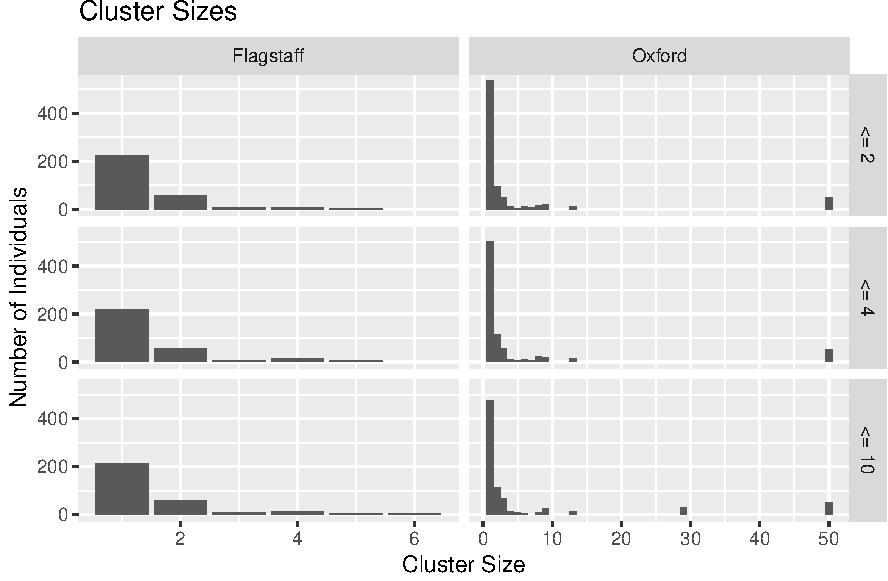
\includegraphics{Paper_files/figure-latex/fig1-1.pdf}
\caption{\label{fig:fig1}Figure 1: Distribution of Cluster Sizes of
Oxfordshire and Flagstaff Data. The row labels denote the threshold
number of SNPs would constitute a cluster.}
\end{figure}

\begin{figure}
\centering
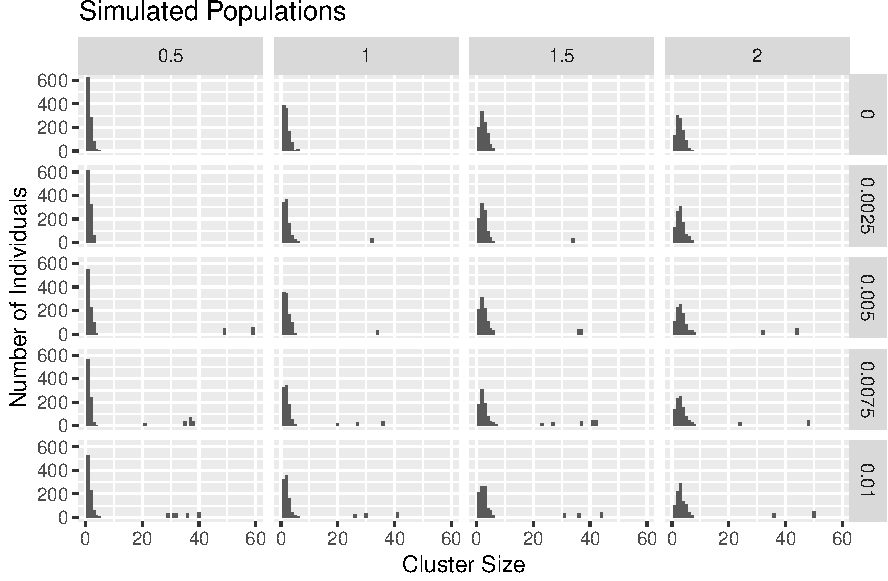
\includegraphics{Paper_files/figure-latex/fig2-1.pdf}
\caption{\label{fig:fig2}Figure 2: Distribution of Cluster Sizes of
Simulated Data. Each column represents the \(\lambda\) parameter of a
Poisson distribution, with larger values representing average larger
cluster sizes among the none extremely large clusters. The rows
represent different levels of mixing in a lognormal distribution and
therefore lower rows have more extremely large clusters.}
\end{figure}

\begin{figure}
\centering
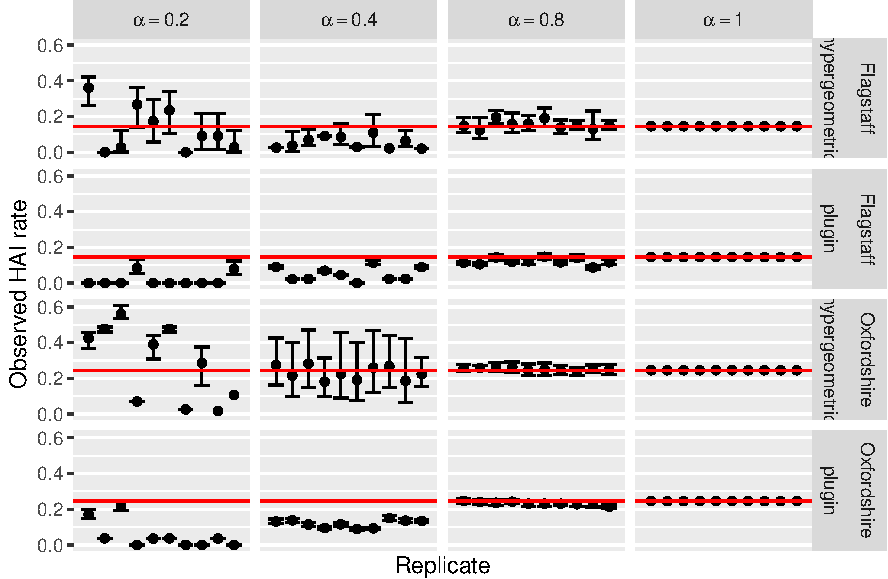
\includegraphics{Paper_files/figure-latex/fig3-1.pdf}
\caption{\label{fig:fig3}Figure 3: Estimators applied to clinical data
sets at different sampling rates. Each graph shows ten replicates Monte
Carlo simulations and associated 95\% confidence interval. The red
horizontal lines display the HAI rate in the full data set.}
\end{figure}

\begin{figure}
\centering
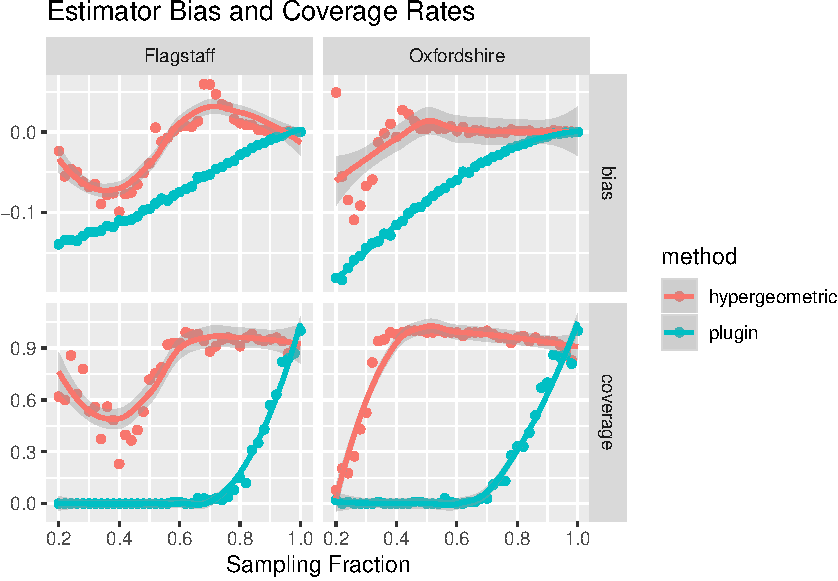
\includegraphics{Paper_files/figure-latex/fig4-1.pdf}
\caption{\label{fig:fig4}Figure 4: Bias and coverage rates at different
sampling fractions for each clinical data set and estimator. The lines
represent the loess smoothed function of the observed values across the
sampling fraction.}
\end{figure}

\begin{figure}
\centering
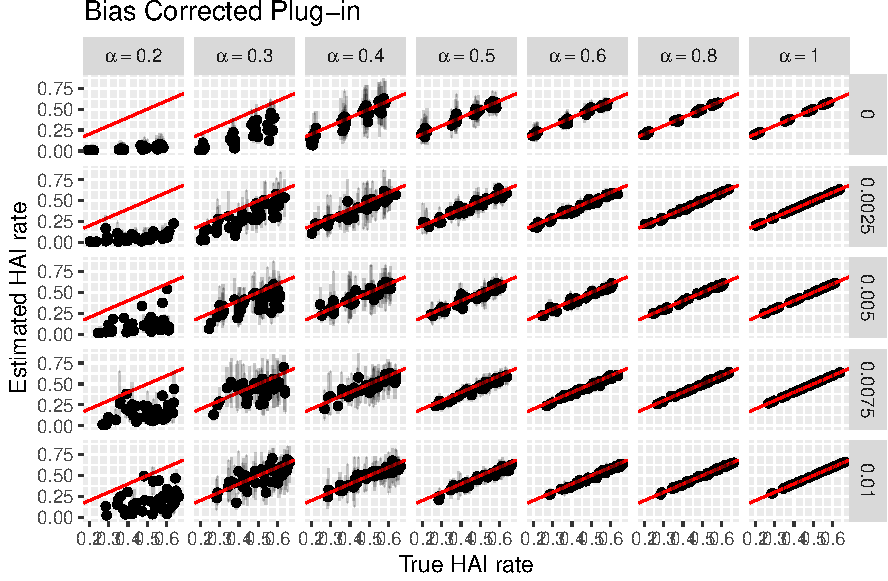
\includegraphics{Paper_files/figure-latex/fig5-1.pdf}
\caption{\label{fig:fig5}Figure 5: Plug-in estimator applied to
simulated data. Columns denote the sampling fraction while rows denote
the mixing fraction with lower rows having more large cluster sizes.}
\end{figure}

\begin{figure}
\centering
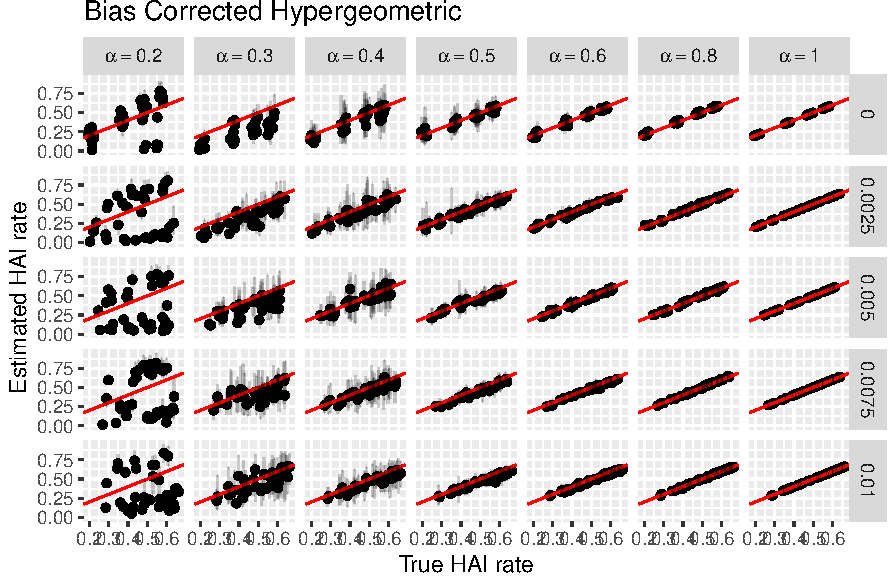
\includegraphics{Paper_files/figure-latex/fig6-1.pdf}
\caption{\label{fig:fig6}Figure 6: Hypergeometric estimator applied to
simulated data. Columns denote the sampling fraction while rows denote
the mixing fraction with lower rows having more large cluster sizes.}
\end{figure}

\hypertarget{refs}{}
\leavevmode\hypertarget{ref-Eyre2013}{}%
1. Eyre DW, Cule ML, Wilson DJ, et al (2013) Diverse Sources of
\textless{}i\textgreater{}C. difficile\textless{}/i\textgreater{}
Infection Identified on Whole-Genome Sequencing. New England Journal of
Medicine 369:1195--1205. \url{https://doi.org/10.1056/NEJMoa1216064}


\end{document}
